\documentclass[11pt,a4paper]{article}
\usepackage[utf8]{inputenc}
\usepackage{amsmath}
\usepackage{amsfonts}
\usepackage{amssymb}
\usepackage{parskip}
\usepackage{tikz}
\usepackage[margin=1in]{geometry}
\usepackage{graphicx}
\usetikzlibrary{arrows,positioning} 
\usepackage{subcaption}
\tikzset{
    %Define standard arrow tip
    >=stealth',
    %Define style for boxes
    punkt/.style={
           circle,
           rounded corners,
           draw=black, thick,
           text width=1em,
           minimum height=1em,
           text centered},
    punktrect/.style={
    rectangle, 
    rounded corners, 
    % fill=black!10,
    draw=black, thick,
    minimum height=1em, 
    text centered},
    % Define arrow style
    pil/.style={punktrect/.style={
    rectangle, 
    rounded corners, 
    % fill=black!10,
    draw=black, very thick,
    text width=10em, 
    minimum height=3em, 
    text centered, 
    on chain},
           ->,
           thick,
           shorten <=2pt,
           shorten >=2pt,}
}


\author{Finnian Lattimore}
\title{A short introduction to causal inference}

\begin{document}
\def\ci{\perp\!\!\!\perp} % from Wikipedia
\newtheorem{theorem}{Theorem}[section]
\newtheorem{definition}{Definition}[section]

\section{Why is causality important}

TODO

(this section should include explanation of why correlation is not causation)

There are two ways in which correlation is not causation. Firstly correlation may not be statistically significant, - ie not even a genuine association. secondly it can be significant but spurious. 


\section{Models of causality}
\label{sec:causalmodels}
To understand causality we first need a more formal definition of what we are talking about. In this section we will look at three slightly different definitions of causality and use them to describe the following very simple example. The aim is to demonstrate the notations and formalisms we will need to tackle more interesting problems later on.

We have developed a new drug for some illness and wish to determine how effective it is. We take a large group of patients and randomly assign half of them to a treatment group and the other half to a control group. The people in the treatment group get the drug, everyone else gets a placebo pill. The question we want to answer is does giving people the active drug improve their changes of recovery relative to giving them the placebo. We will use the variable $X$ (1 = drug, 0 = placebo) to represent the treatment each person receives and $Y$ (1 = recover, 0 = not recover) to describe the outcome .
\subsection{Structural Equation Models}

Structural equation models (SEMs) describe a deterministic world, where underlying mechanisms determine the output of any process for a given input. The mechanism (but not the output) is assumed to be independent of what is fed into it. Linear structural equation models have a long history for causal estimation \cite {Wright1921,Haavelmo1943}. More recently, they have been formalized, generalized to the non-parametric setting and connected to developments in graphical models to provide a powerful causal framework \cite{Pearl2000}.

Mathematically, each variable is a deterministic function of its direct causes and a noise term that captures unmeasured variables. The noise terms are required to be mutually independent. If there is the possibility that an unmeasured variable influences more than one variable of interest in a study, it must be modelled explicitly as a latent (unobserved) variable. Structural equation models can be represented visually as a network. Each variable is a node and arrows are drawn from causes to their effects. For our example the SEM is:

\begin{equation}
\label{eq:SEM}
\begin {aligned}
X = & \epsilon_{x} \\
Y = & f(X,\epsilon_{y})
\end {aligned}
\qquad
\raisebox{-5mm}
{
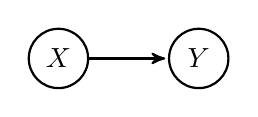
\begin{tikzpicture}[->,>=stealth',shorten >=1pt,auto,node distance=1cm,
  thick,main node/.style={punkt}]

 %nodes
\node[main node](1){$X$};
\node[main node, right=of 1](2){$Y$};


 \path[every node/.style={font=\sffamily\small}]
    (1) edge node {} (2);
	
\end{tikzpicture}
}
\end{equation}

This model encodes the assumption that the outcome $y_{i}$ for an individual $i$ is caused solely by the treatment $x_{i}$ they receive and other factors $\epsilon_{y_{i}}$ that are independent of $X$. This is justifiable on the grounds that $X$ is random; the outcome of a coin flip for each patient should not be related to any of their characteristics (hidden or otherwise). 


The probability of observing $Y$ given $X$, $P(Y = y|X = x) = P(f(x,\epsilon_{y})=y)$ where $\epsilon_{y} ~ P(\epsilon_{y})$ as $\epsilon_{y} \ci \epsilon{x}$  

 

We want to estimate the causal effect of treatment; what is the probability of recovery if we \textbf{take the action} 'treat' versus the \textbf{action} 'placebo'? Taking the action 'treat'  corresponds to replacing the equation $X = \epsilon_{x}$ with $X=1$. The probability distribution over $Y$ given we set $X=1$ is then $P(Y = y|do(X=1)) = P(f(1,\epsilon_{y})=y)$, where we have introduced the $do$ notation to distinguish setting a variable from observing it \cite{Pearl1995}. However, for this model,  The probability of observing $Y$ given $X=1$, $P(Y = y|X = 1)$ is also given by $P(f(1,\epsilon_{y})=y)$ because $\epsilon_{y} \ci \epsilon{x}$. The causal effect is exactly the difference in observed outcomes, as we would intuitively expect for a randomized experiment. In this case, due to the assumption that $X \rightarrow Y$ and that there is no hidden common cause, correlation is causation.  

For a model with $N$ variables, a structural equation model looks like a set of $N$ simultaneous equations, with each variable playing the role of the dependent (left hand side) variable in one equation. However a SEM is, by definition, more than a set of simultaneous equations. By declaring it to be structural we are saying that it represents assumptions about the relationships between variables. When we visualise the model as a network the absence of an arrow between two variables encodes the assumption that one does not cause the other.


\subsection{Causal Bayesian Networks}
\label{sec:causalbayesnets}
Causal Bayesian Networks are, unsurprisingly, an extension of Bayesian networks. Any joint probability distribution can be factorized into a product of conditional probabilities. There are multiple valid factorizations, corresponding to permutations of variable ordering.

\begin{equation}
P(X_{1},X_{2},X_{3},...)=P(X_{1})P(X_{2}|X_{1})P(X_{3}|X_{1},X_{2})...
\end{equation}

We can represent this graphically by drawing a network with a node for each variable and adding links from the variables on the right hand side to the variable on the left for each conditional probability distribution (figure~\ref{fig:bayesnet}). If there are conditional independencies between variables the factorization simplifies, which is reflected by missing edges in the corresponding network. 

\begin{figure}[h]
\centering
\caption{General Bayesian network over 3 variables}
\label{fig:bayesnet}
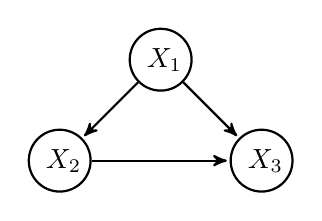
\begin{tikzpicture}[->,>=stealth',shorten >=1pt,auto,node distance=1cm,
  thick,main node/.style={punkt}]

 %nodes
\node[main node](1){$X_{1}$};
\node[main node, below left=of 1](2){$X_{2}$};
\node[main node, below right=of 1](3){$X_{3}$};


 \path[every node/.style={font=\sffamily\small}]
    (1) edge node {} (2)
    	edge node {} (3)
    (2) edge node {} (3);
	
\end{tikzpicture}
\end{figure}

The statement that a given graph $G$ is a Bayesian network for a distribution $P$ tells us that the distribution can be factorized over the nodes and edges in the graph. There can be no missing edges in $G$ that do not correspond to conditional independencies in $P$ (the converse is not true $G$ can have extra edges). If we let $parents_{X_{i}}$ represent the set of variables that are parents of the variable $X_{i}$ in $G$ then we can write the joint distribution as; 

\begin{equation}
P(X_{1}...X_{N}) = \prod_{i = 1...N}P(X_{i}|parents_{X_{i}})
\end{equation}

A causal Bayesian network is a Bayesian network in which it a link $X_{i} \rightarrow X_{j}$, by definition, implies $X_{i}$ causes $X_{j}$. This means that if we intervene and change the value of $X_{i}$, we expect $X_{j}$ to change, but if we intervene to change $X_{j}$, $X_{i}$ will not change. More generally, if $G$ is a causal network for a distribution $P$ defined over variables $X_{1}...X_{N}$, then we can calculate the distribution after an intervention where we set $Z \subset X$ to $z$, denoted $do(Z=z)$ by simply dropping the terms for each of the variables in $Z$ from the factorization given by the network. This is referred to as the truncated product formula \cite{Pearl2000}.

\begin{equation}
\label{eq:truncatedproduct}
 P_{do(Z=z)}(X_{1}...X_{N}) =
  \begin{cases}
  \prod_{i \notin Z}P(X_{i}|parents_{X_{i}}) & \text{if $(X_{1}...X_{N})$ consistant with $Z=z$}  \\
   0       & \text{otherwise } 
  \end{cases}
\end{equation}


Causal Bayesian networks encode information on all interventional distributions over a set of variables. A causal network represents (much) more information than a Bayesian network with identical structure due to the assumption that links can be interpreted causally. Causal Bayesian networks are Bayesian networks so results that apply to Bayesian networks carry directly across;the local markov property states that variables are independent of their non-effects given their direct causes. Similarly the global markov property and d-separation also hold in causal networks. There is an algorithm \cite{Shpitser2012} based on these properties that, for a given network and interventional (do-type) query, can:

a) determine if the query can be translated into an expression involving only distributions over observed variables. In other words, determine if the query is identifiable given the assumptions encoded by the network

b) if it is identiable, return the required expression

Returning at last to our simple example, and phrasing our query in terms of interventions; what would the distribution of outcomes look like if everyone was treated $P(Y|do(X=1))$, relative to if no one was treated $P(Y|do(X=0))$? If we assume that $X$ causes $Y$ and there are no common causes then the causal Bayesian network is just $X \rightarrow Y$, the same structure as the network for the SEM specified by equation (\ref{eq:SEM}). This network represents the (causal) factorization  $P(X,Y) = P(X)P(Y|X)$, so from equation (\ref{eq:truncatedproduct}), $P(Y|do(X)) = P(Y|X)$. In this example, the interventional distribution is equivelent to the observational one as we found earlier using the structural equation model. 

\subsection{Counterfactuals and the Neyman-Rubin framework}

The Neyman-Rubin model \cite{Rubin1974,Rubin1978,Rosenbaum1983, Rubin2005,Rubin2008} defines causality in terms of potential outcomes, or counterfactuals. Counterfactuals are statements about imagined or alternate realities, are prevalent in everyday language and may play a role in the development of causal reasoning in humans \cite{Weisberg2013}. Causal effects are differences in counterfactual variables; what is the difference between what would happen if we did one thing versus what would happen if we did something else. 

In our example, the causal effect of the drug relative to placebo for person $i$ is the difference between what would happen if they were given the drug, denoted $y_{i}^{1}$ versus what would happen if they got the placebo, $y_{i}^{0}$. The fundamental problem of causal inference is that we can only observe one of these two outcomes, since a given person can only be treated or not treated. The problem can be resolved if, instead of people, you have units you can assume are identical or that will revert exactly to their initial state some time after treatment. This type of assumption often holds to a good approximation in the natural sciences and explains why researchers in these fields are less concerned with causal theory. 

Instead of trying to estimate individual effects, lets see if we can learn something about the distributions under treatment or placebo.  Let $Y^{1}$ be a random variable representing the potential outcome if treated. The distribution of $Y^{1}$ is the distribution we would see of $Y$ if everyone was treated. Similarly $Y^{0}$ represents the potential outcome for the placebo. We want to know the difference between the probability of recovery, across the population if everyone was treated, and the probability of recovery given placebo  $P(Y^{1})-P(Y^{0})$. We can estimate, from an experimental or observational study, the probability that people recover if treated $P(Y|X=1)$ and the probability that they recover if not treated $P(Y|X=0)$. Now if $X=0$ then $Y = Y^{0}$. Equivalently stated:

\begin{equation}
\begin{aligned}
P(Y^{0}|X=0)&= P(Y|X=0)\\
P(Y^{1}|X=1)&=P(Y|X=1)
\end{aligned}
\end{equation}

If we assume $X \ci Y^{0}$ and $X \ci Y^{1}$:

\begin{equation}
\begin{aligned}
P(Y^{1}) &= P(Y^{1}|X=1) = P(Y|X=1) \\
P(Y^{0}) &= P(Y^{0}|X=0) = P(Y|X=0) 
\end{aligned}
\end{equation}

\begin{equation}
\implies P(Y^{1})-P(Y^{0}) = P(Y|X=1) - P(Y|X=0)
\end{equation}

The assumptions $X \ci Y^{1}$ and $X \ci Y^{0}$  are referred to as ignoreability assumptions \cite{Rosenbaum1983}. They state that the treatment a each person receives is independent of whether they would recover if treated and if they would recover if not treated. Again this is justified in our example due to the randomization of treatment assignment. In general these assumption do not hold. If people were deciding whether or not to buy the treatment, rather than it being randomly assigned, there could be a variable, for example income,D-separation still applies in the augmented model. that influenced both the decision to get treatment and the likelyhood of recovery given treatment or placebo.



\subsection{Tying it all together. How do these models relate?}

Remarkably for models developed relatively independently in fields with very different approaches and problems, the models we have discussed are definitionally (almost) equivalent. 

If the network for a structural equation model is acyclic, that is if starting from any node and following edges in the direction of the arrows you cannot return to the starting point, then it implies a recursive factorization of the joint distribution over its variables. In other words, the network is a causal Bayesian network. All of the results that apply to causal Bayesian networks also apply to acyclic structural equation models.  Taking an action that sets a variable to a specific value equates to replacing the equation for that variable with a constant. This corresponds to dropping a term in the factorization and the truncated product formula (equation \ref{eq:truncatedproduct}). Thus, the interventional query $P(Y|do(X))$ is identical in these two frameworks. We can also connect this to counterfactuals via:

\begin{equation}
\begin{aligned}
&Y^{0} \equiv P(Y|do(X=0)) \\
&Y^{1} \equiv P(Y|do(X=1))
\end{aligned}
\end{equation}

The assumption $\epsilon_{X} \ci \epsilon_{Y}$, stated for our structural equation model, translates to $X \ci (Y^{0},Y^{1})$ in the language of counterfactuals. When discussing the counterfactual model, we actually made the slightly weaker assumption:

\begin{equation}
\label{eq:weakignore}
X \ci Y^{0} \text{ and } X \ci Y^{1}
\end{equation}

It is possible to relax the independence of errors assumption we made for SEMs slightly to correspond exactly the form of equation (\ref{eq:weakignore}) without losing any of the power provided by d-separation and graphical identification rules \cite{Richardson2013}. To determine if and how an interventional query can be non-parametrically identified, it is equivalent to specify assumptions graphically in terms of functional models or bayesian networks or as conditional independence statements involving counterfactual variables (ignorability assumptions). By non-parametrically, I mean that we are not making any assumptions about the form of the relationships between variables. Models that are not non-parametrically identifiable can still be identified given assumptions about the distributions of variables and the functional relationship between them, for example, that the functions are linear or that the noise is additive \cite{Peters2014}. This form of assumption fits extremely naturally into the structural equation framework. 

We can also pose causal queries that are not interventional and cannot be phrased in terms of the do-notation. Our patients can be broken down into four groups. The first group will recover whether or not they receive treatment, the second group will recover if treated but not on the placebo, the third group will recover on the placebo and not if treated, and the last group will not recover on treatment or placebo. Unfortunately, we don't know which group each person belongs to. Drawing this up as a table:

\begin{tabular}{c|c|c|c}
group & placebo & treatment & probability of group\\
\hline
1 & die & die & $\alpha=P(Y^{0}=0,Y^{1}=0)$\\
2 & die & recover & $\beta=P(Y^{0}=0,Y^{1}=1)$\\
3 & recover & die & $\gamma=P(Y^{0}=1,Y^{1}=0)$\\
4 & recover & recover & $\delta=P(Y^{0}=1,Y^{1}=1)$\\
\end{tabular}

The queries we have been asking thus far are about $P(Y^{0}=1) = \gamma + \delta$ and $P(Y^{1}=1) = \beta + \delta$, but suppose we asked the question; what is the probability that this patient, who was not treated and died, would have recovered if they had been treated? We know they are in either group 1 or 2 since they died without treatment, so the answer is $\frac{\beta}{\alpha+\beta}$. Can we estimate the $\alpha, \beta, \gamma, \delta$ or in other words, identify the joint distribution over the counterfactuals $P(Y^{0},Y^{1})$ given the interventional distributions, $P(Y^{0})$ and $P(Y^{1})$? The answer is no, putting our constraints and unknowns in matrix form:D-separation still applies in the augmented model.

\begin{equation}
\left(
\begin{array}{cccc}
0&0&1&1\\
1&1&0&0\\
0&1&0&1\\
1&0&1&0\\
1&1&1&1\\
\end{array}
\right)
\left(
\begin{array}{c}
\alpha\\
\beta\\
\gamma\\
\delta\\
\end{array}
\right)= 
\left(
\begin{array}{c}
P(Y^{0})\\
1-P(Y^{0})\\
P(Y^{1})\\
1-P(Y^{1})\\
1\\
\end{array}
\right)
\implies
\left(
\begin{array}{c}
\alpha\\
\beta\\
\gamma\\
\delta\\
\end{array}
\right)=
\left(
\begin{array}{c}
1-P(Y^{0})-P(Y^{1})+\delta\\
P(Y^{1})-\delta\\
P(Y^{0})-\delta\\
\delta\\
\end{array}
\right)
\end{equation}
The value of $\delta$ is not determined so the query is not identifiable. However we do get bounds on the terms. Since probabilities cannot be negative, $P(Y{1})-P(Y^{0})-1 \leq \delta \leq min(P(Y^{1}),P(Y^{0})$. Note, if we made the additional assumption $\gamma=0$; that the drug did not cause anyone to die who would otherwise have survived, then we can determine the joint distribution over counterfactuals. Alternatively, if we could assume that after treatment people returned to their initial state after some period of time, (say we were testing a drug for acne) then we could run a crossover study to determine the joint distribution. In a crossover study, the participants are randomly assigned to treatment and placebo, results are measured and then the groups are swapped. The scientific and philosophical validity of counterfactual queries remains under question \cite{Dawid2000,Dawid2014}, however they are nonetheless widely posed in the form of attribution of causal effects to different pathways and mediation \cite{Pearl2014,Imai2010a,VanderWeele2011}. 

There are differences between the models we have considered when it comes to counterfactual queries. Counterfactuals are not defined in causal Bayesian networks, as they only encode information on the interventional distribution over variables.  Counterfactuals can be defined in terms of structural equation models \cite{Pearl2000} but there are subtle differences depending on the form of assumptions made. Structural equation models with independent errors allows the identification of quantities in mediation studies, which are not identifiable with the weak ignorability assumptions and cannot be tested experimentally \cite{Richardson2013}.  

In practice, differences in focus and approach across different fields eclipse these actual differences in the models. The work on causal graphical models \cite{Pearl2000,Sprites} focuses on non-parametric estimation in the population limit and rigorous theoretical foundations. The Neyman-Rubin framework builds on our understanding of randomized experiment and generalizes to quasi-exeperimental and observational settings, with a particular focus on non-random assignment to treatment. This research emphasises estimating average causal effects and provides practical methods for estimation, in particular, propensity scores; a method to control for multiple variables in high dimensional settings with finite data \cite{Rosenbaum1983}. In economics, inferring causal effects from non-experimental data so as to support policy decisions is central to the field. Economists are often interested in broader measures of the distribution of causal effects than the mean and make extensive use of structural equation models, generally with strong parametric assumptions \cite{Heckman2008}. In addition, the parametric structural equation models favoured in economics can be extended to analyse cyclic (otherwise referred to as non-recursive) models. 

The equivalence between models for interventional queries allows researchers to combine the best aspects of all of these models. You can define your assumptions and determine which variables must be controlled for using a graphical model and apply propensity scores to make the adjustment. \cite{Morgan2007} provides an excellent and pragmatic introduction to this combined approach. If non-parametric assumptions are insufficient for identification or lead to overly large uncertainties, you can specify additional assumptions by phrasing your model in terms of structural equations. 


\section{The Do Calculus}
If you state your assumptions in the form of an acyclic structural equation model or a causal bayesian network, the do calculus provides the methodology to determine if a given causal effect can be estimated from observational data and, if it can, provides to formula to do so. The calculus relies heavily on the understanding how conditional independence properties are encoded in bayesian networks. Therefore, in the next section we give a short review of independence in bayesian networks.

\subsection{Independence in bayesian networks: D-separation}

Recall from section \ref{sec:causalbayesnets} the local markov condition: 

\begin{theorem}
\textbf{(Local markov condition)} Given a bayesian network $G$ with nodes $X_{1}...X_{N}$, each variable $X_{i}$ is independent of its non-decendents given its parents in $G$ for all distributions $P(X_{1}...X_{N})$ that are compatible with $G$.
\end{theorem}

The set of conditional independence relations given by the local markov condition can enforce additional independences that also hold in all distributions that are compatible with $G$. D-separation extends the local markov property to find these additional independences and allows us to read from a network if a given conditional independence statement is true in all distributions compatible with that network.

\begin{theorem}
\textbf{(D-separation)} If a set of variables $\boldsymbol{Z}$ d-separates $\boldsymbol{X}$ and $\boldsymbol{Y}$ in $G$ then ${(\boldsymbol{X} \ci \boldsymbol{Y}|\boldsymbol{Z})}$ in all distributions $P$ compatible with $G$. Conversely, if $\boldsymbol{X}$ and $\boldsymbol{Y}$ are d-connected given $\boldsymbol{Z}$ then there will be at least one distribution $P'$ that is compatible with $G$ where they are dependent. 
\end{theorem}

$X$ conditionally independent of $Y$ given $Z$ means, if we know $Z$, learning the value of $Y$ gives us no additional information about $X$. You can also think of this as $Z$ blocks the flow of information from $X$ to $Y$ in the network. Let's examine the four possible bayesian networks over the variables ${X,Y,Z}$ that do not have a direct link  ${X \rightarrow Y}$ (figure \ref{fig:dseptriples}). 

In figure (\ref{fig:dseptripple1}) conditioning on $Z$ renders $X$ and $Y$ conditionally independent. For example, $X$ could be number of years a person smoked, $Z$ the amount of tar in their lungs and $Y$ lung cancer. If you don't know $Z$, knowing how much they smoked changes your estimate of the likelyhood of their having lung cancer, but, if smoking causes cancer purely through the build up of tar in the lungs as we have assumed in this model, then once you measure the amount of tar in the lungs knowing how many years a person smoked for gives you no additional information on the probability that they will develop lung cancer. Figure (\ref{fig:dseptripple2}) is the same as (\ref{fig:dseptripple1}) with $X$ and $Y$ exchanged, which does not change anything since conditional independence is symmetric $(X \ci Y|Z) \Leftrightarrow (Y \ci X|Z)$.

In figure (\ref{fig:dseptripple3}), $Z$ could represent having an illness and $X$ and $Y$ could be two independent tests that can detect (with some error) that illness. Without conditioning on $Z$ you would expect results from the two different tests to be highly correlated, but if you already know someone has the illness then learning they tested positive to the test $X$ doesn't change the likelyhood they test positive in test $Y$. Again, conditioning on $Z$ blocks the path from $X$ to $Y$.

The arrangement of variables in figure (\ref{fig:dseptripple4}), often referred to as a collider or v-structure, is the odd one out. In this case $X$ is independent of $Y$ without conditioning on $Z$ but if you do condition on $Z$ then $X$ and $Y$ actually become dependent. Suppose $X$ is socio-economic status, $Y$ is gender and $Z$ is receipt of a scholarship available to female or disadvantaged students. Roughly equal numbers of women and men grow up in poorer families so $X$ is independent of $Y$, but if you know that a given student received a scholarship, then learning that they are male tells you they must have a low socio-economic background. Conditioning on $Z$ unblocks the path from $X$ to $Y$. 


\begin{figure}[h]
\centering
\caption{All possible two edge paths from $X$ to $Y$ via $Z$}
\label{fig:dseptriples}
\begin{subfigure}[t]{0.2\textwidth}
\centering
\caption{$X \ci Y| Z$}
\label{fig:dseptripple1}
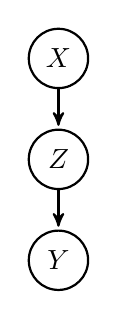
\begin{tikzpicture}[->,>=stealth',shorten >=1pt,auto,node distance=.5cm,
  thick,main node/.style={punkt}]
\node[main node](1){$X$};
\node[main node, below =of 1](2){$Z$};
\node[main node, below =of 2](3){$Y$};
 \path[every node/.style={font=\sffamily\small}]
    (1) edge node {} (2)
    (2) edge node {} (3);	
\end{tikzpicture}
\end{subfigure}
\begin{subfigure}[t]{0.2\textwidth}
\centering
\caption{$X \ci Y|Z$}
\label{fig:dseptripple2}
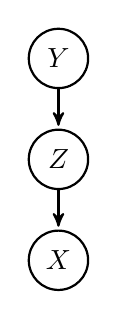
\begin{tikzpicture}[->,>=stealth',shorten >=1pt,auto,node distance=.5cm,
  thick,main node/.style={punkt}]
\node[main node](1){$Y$};
\node[main node, below =of 1](2){$Z$};
\node[main node, below =of 2](3){$X$};
 \path[every node/.style={font=\sffamily\small}]
    (1) edge node {} (2)
    (2) edge node {} (3);	
\end{tikzpicture}
\end{subfigure}
\begin{subfigure}[t]{0.2\textwidth}
\centering
\caption{$X \ci Y|Z$}
\label{fig:dseptripple3}
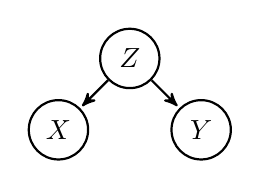
\begin{tikzpicture}[->,>=stealth',shorten >=1pt,auto,node distance=.5cm,
  thick,main node/.style={punkt}]
\node[main node](1){$Z$};
\node[main node, below left =of 1](2){$X$};
\node[main node, below right=of 1](3){$Y$};
 \path[every node/.style={font=\sffamily\small}]
    (1) edge node {} (2)
        edge node {} (3);	
\end{tikzpicture}
\end{subfigure}
\begin{subfigure}[t]{0.2\textwidth}
\centering
\caption{$X \ci Y|\{\}$}
\label{fig:dseptripple4}
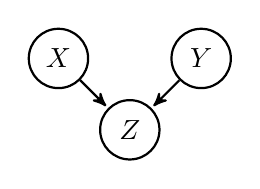
\begin{tikzpicture}[->,>=stealth',shorten >=1pt,auto,node distance=.5cm,
  thick,main node/.style={punkt}]
\node[main node](1){$Z$};
\node[main node, above left =of 1](2){$X$};
\node[main node, above right =of 1](3){$Y$};
 \path[every node/.style={font=\sffamily\small}]
    (2) edge node {} (1)
    (3) edge node {} (1);	
\end{tikzpicture}
\end{subfigure}
\end{figure}

For a general bayesian network a path between two variables may involve more than three variables. 

\begin{definition}
\textbf{(unblocked path)} A path from $X$ to $Y$ is a sequence of edges linking adjacent nodes starting at $X$ and finishing at $Y$,  $(X,V_{1},V_{2}...V_{k},Y)$. It is unblocked if every triple, $X-V_{1}-V_{2},V_{1}-V_{2}-V{3},...,V_{k-1}-V_{k}-Y$ in the path is unblocked (each triple will belong to one of the cases in figure \ref{fig:dseptriples})
\end{definition}

If all paths between two nodes are blocked by conditioning on $\boldsymbol{Z}$ then no information can flow between them and they are d-separated given $\boldsymbol{Z}$. 

\begin{definition}
The variables $\boldsymbol{X}$ are d-separated from $\boldsymbol{Y}$ given $\boldsymbol{Z}$ in the network $G$ if, after conditioning on $\boldsymbol{Z}$ there are no unblocked paths from $\boldsymbol{X}$ to $\boldsymbol{Y}$.  
\end{definition}

For a more complete introduction to d-separation (with proofs) see \cite{Koller2009}.

\subsection{The three rules}
The do calculus consists of three rules. They derive from the causal information encoded in a causal network and the properties of d-separation and do not imply any addition assumptions other than that of specifying the causal network. The key property of these three rules is that they are complete. If an interventional (do-type) query can be transformed to a do-less statement via repeated application of these rules we can get an unbiased point estimate of the causal effect from observational data. Conversely, if the query is not identified via these rules we cannot get an unbiased estimate of the causal effect without additional assumptions, even with an infinite amount of observational data. 

\subsubsection{Rule 1}
This rule describes which variables, on which we have not intervened, effect the distribution of the outcome given some intervention. The intervention $do(\boldsymbol{X}=\boldsymbol{x})$ changes a causal network, $G$, in a simple way. Variables in $\boldsymbol{X}$ are no longer determined by their parents but instead take on fixed values specified by $\boldsymbol{x}$. This corresponds to deleting the edges with arrows into variables in $\boldsymbol{X}$  (see figure \ref{fig:mutilatednet}). The resulting 'mutilated' network $G_{\overline{\boldsymbol{X}}}$ remains a causal network and d-separation still applies. 

If $(\boldsymbol{Y} \ci \boldsymbol{W} | \boldsymbol{Z},\boldsymbol{X})$ in $G_{\overline{\boldsymbol{X}}}$:
\begin{equation}
\label{eq:Do1}
 P(\boldsymbol{Y}|do(\boldsymbol{X}=\boldsymbol{x}),\boldsymbol{Z}=\boldsymbol{z},\boldsymbol{W}=\boldsymbol{w}) = P(\boldsymbol{Y}|do(\boldsymbol{X}=\boldsymbol{x}),\boldsymbol{Z}=\boldsymbol{z}) 
\end{equation}

$\implies$ if $(\boldsymbol{Y} \ci \boldsymbol{W} | \boldsymbol{X})$ in $G_{\overline{\boldsymbol{X}}}$:
\begin{equation}
\label{eq:Do12}
 P(\boldsymbol{Y}|do(\boldsymbol{X}=\boldsymbol{x}),\boldsymbol{W}=\boldsymbol{w}) = P(\boldsymbol{Y}|do(\boldsymbol{X}=\boldsymbol{x})) 
\end{equation}

This stems directly from the fact that the relationship between d-separation in a network and independence in the corresponding probability distribution still holds in the mutilated network. 

\begin{figure}[h]
\centering
\caption{Intervention in a causal bayesian network}
\label{fig:mutilatednet}
\begin{subfigure}[t]{0.3\textwidth}
\centering
\caption{original network, $G$}
\label{fig:mutilatedOriginal}
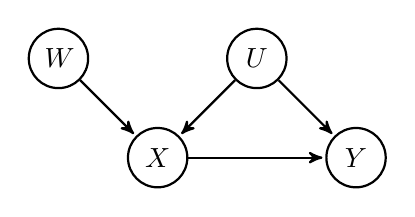
\begin{tikzpicture}[->,>=stealth',shorten >=1pt,auto,node distance=1cm,
  thick,main node/.style={punkt}]

 %nodes
\node[main node](1){$U$};
\node[main node, below left=of 1](2){$X$};
\node[main node, below right=of 1](3){$Y$};
\node[main node, above left=of 2](4){$W$};


 \path[every node/.style={font=\sffamily\small}]
    (1) edge node {} (2)
    	edge node {} (3)
    (2) edge node {} (3)
    (4) edge node {} (2);
	
\end{tikzpicture} 
\end{subfigure}
\begin{subfigure}[t]{0.5\textwidth}
\centering
\caption{network after the intervention $do(X=x)$, $G_{\overline{X}}$}
\label{fig:mutilatedAfter}
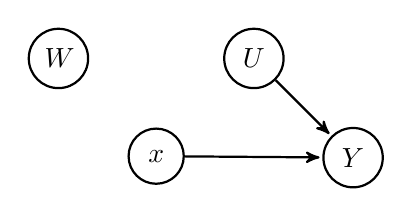
\begin{tikzpicture}[->,>=stealth',shorten >=1pt,auto,node distance=1cm,
  thick,main node/.style={punkt}]

 %nodes
\node[main node](1){$U$};
\node[main node, below left=of 1](2){$x$};
\node[main node, below right=of 1](3){$Y$};
\node[main node, above left=of 2](4){$W$};


 \path[every node/.style={font=\sffamily\small}]
    (1) edge node {} (3)
    (2) edge node {} (3);
    
\end{tikzpicture}
\end{subfigure}
\end{figure}

\subsubsection{Rule 2}
Rule 2 states when conditioning on $\boldsymbol{X} = \boldsymbol{x}$ and intervening  $do(\boldsymbol{X}=\boldsymbol{x})$ have the same effect on the distribution of the outcome $\boldsymbol{Y}$. You can think of this as when correlation is causation. It is easiest to understand by explicitly including the intervention process in the graphical model. We can depict the possibility of intervention by adding a new decision node $\hat{X}$ as a parent of each $X$ in the set of nodes we are intervening on (figure \ref{fig:augmentedNetwork}). Let $\epsilon$ be some arbitrary value not in the set of possible values for $X$. If $X = \epsilon$ the distribution of $X$ is what it was without intervention. Otherwise, if $X=x$, $X$ deterministically takes the value $x$ and is independent of its previous parents, representing the intervention $do(X=x)$. We use the notation $G^{\dagger}$ to represent $G$ augmented with these decision nodes. 

if $(\boldsymbol{Y} \ci \boldsymbol{\hat{X}}|\boldsymbol{X},\boldsymbol{Z},\boldsymbol{W})$ in $G^{\dagger}_{\boldsymbol{\overline{Z}}}$:

\begin{equation}
\label{eq:Do2}
P(\boldsymbol{Y}|do(\boldsymbol{Z}=\boldsymbol{z}),do(\boldsymbol{X}=\boldsymbol{x}),\boldsymbol{W}=\boldsymbol{w}) = P(\boldsymbol{Y}|do(\boldsymbol{Z}=\boldsymbol{z}),\boldsymbol{X}=\boldsymbol{x},\boldsymbol{W}=\boldsymbol{w})
\end{equation}

$\implies$ if  $(\boldsymbol{Y} \ci \boldsymbol{\hat{X}}|\boldsymbol{X})$ in $G^{\dagger}$:
\begin{equation}
\label{eq:Do22}
P(\boldsymbol{Y}|do(\boldsymbol{X}=\boldsymbol{x})) = P(\boldsymbol{Y}|\boldsymbol{X}=\boldsymbol{x})
\end{equation}

If the outcome does not depend on how the decision to assign the interventional variables was made, then the interventional distribution equals the observational one. 

\begin{figure}[h]
\centering
\caption{Augmentated causal network with intervention}
\label{fig:augmentedNetwork}
\begin{subfigure}[t]{0.4\textwidth}
\centering
\caption{original network, $G$}
\label{fig:augmentedOriginal}
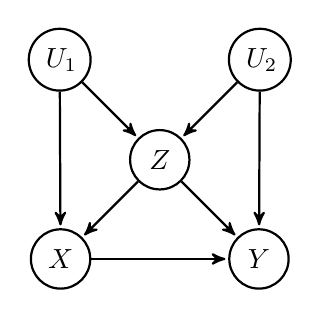
\begin{tikzpicture}[->,>=stealth',shorten >=1pt,auto,node distance=1cm,
  thick,main node/.style={punkt}]
 %nodes
\node[main node](1){$Z$};
\node[main node, below left=of 1](2){$X$};
\node[main node, below right=of 1](3){$Y$};
\node[main node, above left = of 1](4){$U_{1}$};
\node[main node, above right = of 1](5){$U_{2}$};


 \path[every node/.style={font=\sffamily\small}]
 	(2) edge node {} (3)
 	(4) edge node {} (2)
 		edge node {} (1)
 	(5) edge node {} (3)
 		edge node {} (1)
 	(1) edge node {} (2)
 		edge node {} (3);
    
	
\end{tikzpicture} 
\end{subfigure}
\begin{subfigure}[t]{0.4\textwidth}
\centering
\caption{augmented network after the intervention $do(Z=z)$, $G^{\dagger}_{\overline{Z}}$}
\label{fig:augmentedAfter}
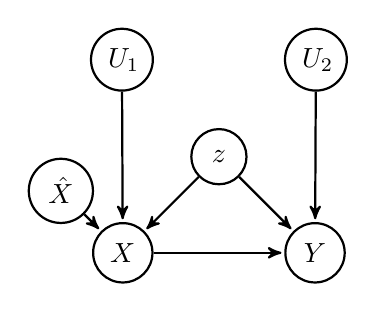
\begin{tikzpicture}[->,>=stealth',shorten >=1pt,auto,node distance=0.3cm,
  thick,main node/.style={punkt}]

\node[main node](1){$z$};
\node[below left=of 1](2){};
\node[below right=of 1](3){};
\node[main node, below left=of 2](4){$X$};
\node[main node, below right=of 3](5){$Y$};
\node[above right=of 1](6){};
\node[above left=of 1](7){};
\node[main node, above left=of 7](8){$U_{1}$};
\node[main node, above right=of 6](9){$U_{2}$};
\node[main node, above left=of 4](10){$\hat{X}$};


 \path[every node/.style={font=\sffamily\small}]
 	(4) edge node {} (5)
 	(10) edge node {} (4)
 	(8) edge node {} (4)
 	(9) edge node {} (5)
 	(1) edge node {} (4)
 		edge node {} (5);
 	
    
\end{tikzpicture}
\end{subfigure}
\end{figure}

\subsubsection{Rule 3}
This rule describes cases where the intervention $do(\boldsymbol{X}=\boldsymbol{x})$ has no effect on the distribution of the outcome $\boldsymbol{Y}$. 

if $(\boldsymbol{Y} \ci \boldsymbol{\hat{X}} |\boldsymbol{Z},\boldsymbol{W})$ in $G^{\dagger}_{\boldsymbol{\overline{Z}}}$:
\begin{equation}
\label{eq:Do3}
P(\boldsymbol{Y}|do(\boldsymbol{Z}=\boldsymbol{z}),do(\boldsymbol{X}=\boldsymbol{x}),\boldsymbol{W}=\boldsymbol{w}) = P(\boldsymbol{Y}|do(\boldsymbol{Z}=\boldsymbol{z}),\boldsymbol{W}=\boldsymbol{w})
\end{equation}
$\implies$ if  $(\boldsymbol{Y} \ci \boldsymbol{\hat{X}})$ in $G^{\dagger}$:
\begin{equation}
\label{eq:Do32}
P(\boldsymbol{Y}|do(\boldsymbol{X}=\boldsymbol{x})) = P(\boldsymbol{Y})
\end{equation}
The statement that $\boldsymbol{Y} \ci \boldsymbol{\hat{X}}$ without conditioning on $\boldsymbol{X}$ implies that there is no unblocked path from $\boldsymbol{X}$ to $\boldsymbol{Y}$ which starts on an arrow leaving $\boldsymbol{X}$. This means there is no causal effect of $\boldsymbol{X}$ on $\boldsymbol{Y}$ and the intervention $do(\boldsymbol{X}=\boldsymbol{x})$ does not alter the distribution of $P(\boldsymbol{Y})$.

\subsection{Easy graphical tests for identifiability}
Determining if a network is identifiable via the two calculus still requires some algebra and it may not always be obvious what sequence of rules are required for a given network. From the do-calculus we can derive some quick graphical tests that are sufficient (but not necessary) for non-parametric identifiability, and align with intuitive ideas about estimating causal effect by adjusting for confounding variables. 

\subsubsection{If all variables are observed}
If all the variables in a causal network can be measured any interventional query on that network are identifiable. You just have to condition on the parents of the variables on which you intervene. For discrete variables, the causal effect is given by:

\begin{equation}
P(\boldsymbol{Y}|do(\boldsymbol{X})) = \sum_{\boldsymbol{Pa_{X}}}{P(\boldsymbol{Y}|\boldsymbol{X},\boldsymbol{Pa_{X}})P(\boldsymbol{Pa_{X}})}
\end{equation}

where $\boldsymbol{Pa_{X}}$ are the parents of $\boldsymbol{X}$.


Conditioning on the parents blocks all information that does not flow causally (along the arrows) from the variables on which we intervened which eliminates spurious correlations and gives the causal effect. 

\subsubsection{The Back Door criterion}
The back door criterion generalizes from the case where all variables can be measured by observing we don't need to condition on all the parents of the intervened on variables: it is sufficient to condition on a set of variables that block all spurious paths from $\boldsymbol{X}$ to $\boldsymbol{Y}$. A spurious, or back door, path is one that leaves $\boldsymbol{X}$ against the direction of the causal arrows. If we have a set of variables $\boldsymbol{Z}$ that block all back door paths from $\boldsymbol{X}$ to $\boldsymbol{Y}$, where no variable in $\boldsymbol{Z}$ is a descendent of $\boldsymbol{X}$ then:

\begin{equation}
P(\boldsymbol{Y}|do(\boldsymbol{X})) = \sum_{Z}{P(\boldsymbol{Y}|\boldsymbol{X},\boldsymbol{Z})P(\boldsymbol{Z})}
\end{equation}

The requirement that $\boldsymbol{Z}$ should not include descendants of $\boldsymbol{X}$ stems from the fact that we don't want to open any new spurious paths. If $Z$ descends from $X$ then it may lie on a path of the form $X \rightarrow...\rightarrow Z \leftarrow... Y$, which conditioning on $Z$ would open. The back door criterion corresponds exactly to the strong ignoreability assumption \cite{Rosenbaum1983}, used to justify the validity of a causal estimate in the counterfactual approach . If $\boldsymbol{Z}$ satisfies the backdoor criterion then, for a single binary treatment variable $X$ and outcome variable $Y$, $\{Y^{0},Y^{1}\} \ci X | \boldsymbol{Z}$. 
 
\subsubsection{The Front Door Criterion}
It we have an unobservable variable creating a spurious path from $\boldsymbol{X}$ to $\boldsymbol{Y}$ then we cannot apply the back door criterion to directly estimate $P(\boldsymbol{Y}|do(\boldsymbol{X}))$. However, if there is a set of mediating variables $\boldsymbol{M}$ that intercepts all all the direct (non-spurious) paths from $\boldsymbol{X}$ to $\boldsymbol{Y}$ and we can estimate the causal effect of $\boldsymbol{X}$ on $\boldsymbol{M}$ and the causal effect of $\boldsymbol{M}$ on $\boldsymbol{Y}$ then we can combine these terms to get the causal effect of $\boldsymbol{X}$ on $\boldsymbol{Y}$. 

\begin{equation}
\begin {aligned}
P(\boldsymbol{Y}|do(\boldsymbol{X})) & = \sum_{\boldsymbol{M}}{P(\boldsymbol{M}|do(\boldsymbol{X}))P(\boldsymbol{Y}|do(\boldsymbol{M}))} \\
&= \sum_{\boldsymbol{M}}{P(\boldsymbol{M}|\boldsymbol{X})} \sum_{\boldsymbol{X}}P(\boldsymbol{Y}|\boldsymbol{X},\boldsymbol{M})P(\boldsymbol{X}) 
\end {aligned}
\end{equation}

\subsubsection{Examples}

We are now in a position to consider some more interesting examples than the one in section \ref{sec:causalmodels}. Consider the question; does eating chocolate increase or decrease the risk of obesity? Assume we have data from a cross-sectional study where a large group of people were weighed and asked how much chocolate they ate. It is easy to come up with a whole lot of variables that may causally effect chocolate consumption and obesity, ie. age, income and gender, so we cannot conclude that the causal effect is equivalent to the correlation. If we assume there may be unknown variables (denoted by $U$ in all the following examples) that effect both obesity and chocolate consumption, (figure \ref{fig:chockNI}), the causal effect cannot be identified as there is no way to block the spurious path through the unobserved variables. If we assume the only confounding variables are income, age and gender, (figure \ref{fig:chockI}), we can calculate the causal effect by conditioning on these variables.  


\begin{figure}[h]
\centering
\caption{Chocolate and Obesity}
\label{fig:chocolate}
\begin{subfigure}[t]{0.4\textwidth}
\caption{Not identifiable}
\label{fig:chockNI}
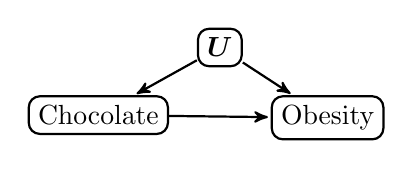
\begin{tikzpicture}[->,>=stealth',shorten >=1pt,auto,node distance=0.5cm,  thick,main node/.style={punktrect}]

 %nodes
\node[main node](1){$\boldsymbol{U}$};
\node[main node, below left=of 1](2){Chocolate};
\node[main node, below right=of 1](3){Obesity};


 \path[every node/.style={font=\sffamily\small}]
    (1) edge node {} (2)
    	edge node {} (3)
    (2) edge node {} (3);
\end{tikzpicture}
\end{subfigure}
\begin{subfigure}[t]{0.4\textwidth}
\caption{Identifiable}
\label{fig:chockI}
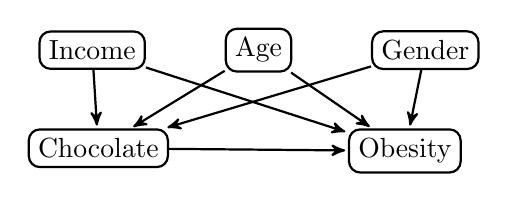
\begin{tikzpicture}[->,>=stealth',shorten >=1pt,auto,node distance=1cm,  thick,main node/.style={punktrect}]

 %nodes
\node[main node](1){Age};
\node[main node, left= of 1](4){Income};
\node[main node, right=of 1](5){Gender};
\node[main node, below left=of 1](2){Chocolate};
\node[main node, below right=of 1](3){Obesity};

 \path[every node/.style={font=\sffamily\small}]
    (1) edge node {} (2)
    	edge node {} (3)
    (2) edge node {} (3)
    (4) edge node {} (2)
        edge node {} (3)
    (5) edge node {} (2)
    	edge node {} (3);
\end{tikzpicture}
\end{subfigure}
\end{figure}

In reality of course there are many other variables involved  \cite{Golomb2012} and it may not be obvious from prior knowledge or theory what role the variables play in the network. This is important as conditioning on the wrong variables can increase the bias in a causal estimate: Conditioning on a collider variable, $\rightarrow Z \leftarrow$, may open a previously blocked, spurious path \cite{Sjolander2009a} (figure \ref{fig:colliderCondition}) . Conditioning on a variable that mediates between the cause and effect biases the causal estimate by blocking a true casual path (figure \ref{fig:mediationBias}). Conditioning on a variable that is a true confounder, that is a common cause of both $X$ and $Y$, may increase the bias in our causal estimate if it moves the causal estimate in the opposite direction than would correcting for a hidden (and stronger) confounder $U$. Finally, (although it is not obvious graphically) conditioning on a variable that is a cause of $X$ but not (or only weakly) a cause of $Y$ can amplify or introduce bias \cite{Pearl2012b,Wooldridge2009}.


\begin{figure}[]
		\caption{Conditioning on a collider variable can introduce bias}\label{fig:colliderCondition}
       \centering
        \begin{subfigure}[t]{0.4\textwidth}
        \centering
                \caption{post-treatment bias: conditioning on $Z$ opens the spurious path $X,Z,Y$}
                \label{fig:postTreatmentBias}
                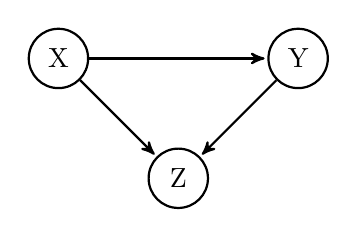
\begin{tikzpicture}[->,>=stealth',shorten >=1pt,auto,node distance=1cm,  thick,main node/.style={punkt}]
 %nodes
\node[](1){}; 
\node[main node, left = of 1](2){X};
\node[main node, right= of 1](3){Y};
\node[main node, below =of 1](4){Z};
 \path[every node/.style={font=\sffamily\small}]
    (2) edge node {} (3)
    	edge node {} (4)
    (3) edge node {} (4);
\end{tikzpicture}
        \end{subfigure}%
        ~ %add desired spacing between images, e. g. ~, \quad, \qquad, \hfill etc.
          %(or a blank line to force the subfigure onto a new line)
        \begin{subfigure}[t]{0.4\textwidth}
        \centering
                \caption{M-bias: conditioning on $Z$ opens the path $X,U_{1},Z,U_{2},Y$}
                \label{fig:Mbias}
                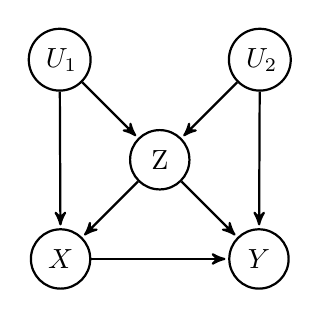
\begin{tikzpicture}[->,>=stealth',shorten >=1pt,auto,node distance=1cm,  thick,main node/.style={punkt}]
 %nodes
\node[main node](1){Z}; 
\node[main node, below left = of 1](2){$X$};
\node[main node, below right= of 1](3){$Y$};
\node[main node, above left = of 1](5){$U_{1}$};
\node[main node, above right = of 1](6){$U_{2}$};
 \path[every node/.style={font=\sffamily\small}]
    (2) edge node {} (3)
    (5) edge node {} (1)
    	edge node {} (2)
    (6) edge node {} (1)
    	edge node {} (3)
    (1) edge node {} (2)
    	edge node {} (3);
\end{tikzpicture}
        \end{subfigure}    
\end{figure}


\begin{figure}[]
\centering
\caption{Conditioning on a mediating variable ($Z$) can introduce bias}
\label{fig:mediationBias}
 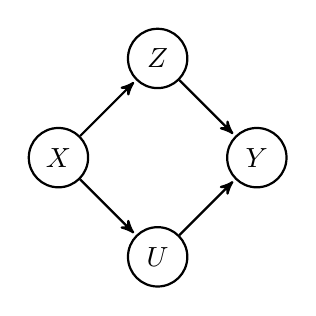
\begin{tikzpicture}[->,>=stealth',shorten >=1pt,auto,node distance=1cm,  thick,main node/.style={punkt}]
 %nodes
\node[main node](1){$X$}; 
\node[main node, above right = of 1](2){$Z$};
\node[main node, below right= of 1](3){$U$};
\node[main node, above right = of 3](4){$Y$};
\path[every node/.style={font=\sffamily\small}]
	(1) edge node {} (2)
		edge node {} (3)
	(2) edge node {} (4)
	(3) edge node {} (4);
  
\end{tikzpicture}
\end{figure}

\begin{figure}[]
\centering
\caption{Conditioning on a confounder ($Z$) can increase bias}
\label{fig:biasAmplification}
 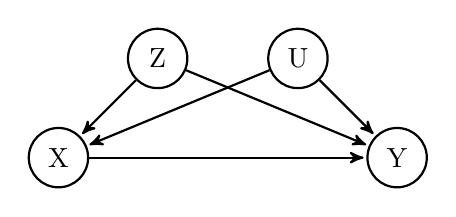
\begin{tikzpicture}[->,>=stealth',shorten >=1pt,auto,node distance=1cm,  thick,main node/.style={punkt}]
 %nodes
\node[main node](1){Z}; 
\node[main node, below left = of 1](2){X};
\node[main node, right = of 1](4){U};
\node[main node, below right= of 4](3){Y};

 \path[every node/.style={font=\sffamily\small}]
    (2) edge node {} (3)
    (1) edge node {} (2)
    	edge node {} (3)
    (4) edge node {} (2)
    	edge node {} (3);
    
\end{tikzpicture}
\end{figure}

\begin{figure}[]
\centering
\caption{Bias amplification}
\label{fig:biasAmplification}
\begin{subfigure}[t]{0.4\textwidth}
\centering
\caption{Conditioning on an instrumental variable $Z$ can increase bias in estimate of effect of $X$ on $Y$}
\label{fig:instrumentalBias}
 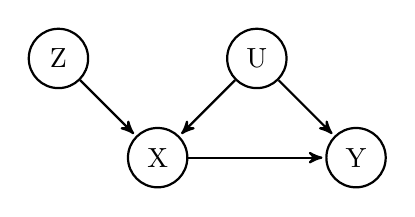
\begin{tikzpicture}[->,>=stealth',shorten >=1pt,auto,node distance=1cm,  thick,main node/.style={punkt}]
 %nodes
\node[main node](1){U}; 
\node[main node, below left = of 1](2){X};
\node[main node, below right = of 1](3){Y};
\node[main node, above left= of 2](4){Z};

 \path[every node/.style={font=\sffamily\small}]
    (2) edge node {} (3)
    (1) edge node {} (2)
    	edge node {} (3)
    (4) edge node {} (2);
    
\end{tikzpicture}
\end{subfigure}
 \begin{subfigure}[t]{0.4\textwidth}
\centering
\caption{Conditioning on a confounding variable that is strongly linked to $X$ and weakly linked to $Y$ can increase bias.}
\label{fig:semiinstrumentalbias}

 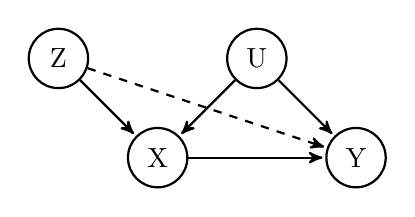
\begin{tikzpicture}[->,>=stealth',shorten >=1pt,auto,node distance=1cm,  thick,main node/.style={punkt}]
 %nodes
\node[main node](1){U}; 
\node[main node, below left = of 1](2){X};
\node[main node, below right = of 1](3){Y};
\node[main node, above left= of 2](4){Z};

 \path[every node/.style={font=\sffamily\small}]
    (2) edge node {} (3)
    (1) edge node {} (2)
    	edge node {} (3)
    (4) edge node {} (2)
    	edge [dashed] node {} (3);
    	

\end{tikzpicture}
\end{subfigure}
\end{figure}


For some problems, the temporal ordering of events imposes restrictions on the causal structure. Consider the example of a non-randomized trial. A new treatment is developed and made available to a large group of patients some of whom decide to take. Researchers have variables on the health, income, gender, age, etc of the patients before the treatment was offered (pre-treatment variables) and collect further data on the health of all patients after treatment has begun (post-treatment variables). It has been understood for a long time that conditioning on post-treatment variables can increase bias \cite{Rosenbaum1984a}. The realization that that conditioning on pre-treatement can also introduce bias is more recent. Not conditioning on post-treatment variables avoids the biases in figure \ref{fig:postTreatmentBias} and figure \ref{fig:mediationBias}. However, M-bias (figure \ref{fig:Mbias}) and bias amplification (figure \ref{fig:biasAmplification}) are consequences of conditioning on pre-treatment variables. 


It is clear we need to be wary of the condition on everything approach and the condition on all pre-treatment variables approach. But what is the alternative if the structure of the causal network is not clear from prior knowledge? One approach would be to construct a number of different plausible structures and evaluate the desired causal effect for each of them. This would give more accurate uncertainty bounds for the causal effect. Alternatively, one could apply a causal discovery algorithm (see section \ref{sec:causaldiscovery}). 

It may be that there are some general conditions under which certain types of biases are less likely or weaker than other. For example, in the situation in figure \ref{fig:Mbias}, where $Z$ is both a confounding variable and part of an M-structure. Conditioning on $Z$ blocks the spurious path $X \leftarrow Z \rightarrow Y$ and opens the spurious path $X \leftarrow U_{1} \rightarrow Z \leftarrow U_{2} \rightarrow Y$. Should we condition on $Z$ or not? Under what general assumptions is one of these paths weaker than the other. There has been relatively little work in this area. \cite{Vansteelandt2012} gives a description of the problem and links it to selecting covariates when the goal is causal estimation. \cite{Myers2011, Pearl2012b} consider if one should adjust for a variable that could be either an instrumental variable or a confounder for the effect of $X$ on $Y$. 


\section{It's not (non-parametrically) identifiable! What can I do?}
\subsection{Bounding causal effects}
Causal effects that cannot be identified can often still be bounded. In other words, bounds require weaker assumptions than point identification.
 
\subsection{Additional assumptions}
additive noise
causal anti-causal \cite{Janzing2012}
learning what indicates causality. 

\subsection{Instrumental variables}



\section{Causal structure learning (causal discovery)}
\label{sec:causaldiscovery}
If you have a method for doing things pairwise, then you can extend it to a full network. 

peters approach \cite{Peters2014}
Pearl/Verma/Sprites approach \cite{Pearl2000} 


\section{Causality and prediction}
Refresh the difference between a causal query and predictive query.
Point out the importance of accurate prediction for causal inference. For example, if we can predict the control response, we can run experimental studies without controls (\cite{Brodersen2013})


\bibliographystyle{plain}% Select the citation style e.g. ieeetr
\bibliography{library}% write the directory to the .bib file
\end{document}








